%----------------------------------------------------------------------------------------
%	PACKAGES AND OTHER DOCUMENT CONFIGURATIONS
%----------------------------------------------------------------------------------------

\documentclass[letter,11pt]{scrartcl}

% Fonts, Line-Spacing, and Indentation
\usepackage{fourier}
\usepackage[T1]{fontenc}
\usepackage{microtype}
\usepackage{color}
\setlength\parindent{0pt}
\usepackage{booktabs}
\usepackage{hyperref}
\usepackage{titlesec}
\usepackage[hang,small,labelfont=bf,up,textfont=it,up]{caption}

%------------------------------------------------------

% Symbols
\usepackage{amssymb,amsmath,amsthm}
\usepackage{MnSymbol}
\usepackage{lambda}
\renewcommand{\progfontsize}{\normalsize}
\providecommand{\abs}[1]{\lvert#1\rvert}
\providecommand{\norm}[1]{\lVert#1\rVert}

%------------------------------------------------------

% Sections and Margins
\usepackage{chngcntr}
\usepackage{scrextend}

%------------------------------------------------------

% Venn Diagrams and Images
\usepackage{tikz}
\usetikzlibrary{arrows,backgrounds,petri,shapes,topaths}
\usepackage{float}
\usepackage{wrapfig}

%------------------------------------------------------

% Margins
\usepackage[hmarginratio=1:1,top=10mm,columnsep=20pt]{geometry}

%------------------------------------------------------

% Custom Theorem Setup
\newtheorem{innercustomthm}{Theorem}
\newenvironment{customthm}[1]
  {\renewcommand\theinnercustomthm{#1}\innercustomthm}
  {\endinnercustomthm}


%------------------------------------------------------

% Custom macros
\newcommand{\inlinecode}{\texttt}


%----------------------------------------------------------------------------------------
%	TITLE SECTION
%----------------------------------------------------------------------------------------

\title{
  \normalfont \normalsize
  \textsc{Data Structures - CS 261 (Spring 2015)} \\
  \huge Assignment \#6 -- Questions
}

\author{Keeley Abbott
\\ Theodore Duchow-Pressley}

\date{\normalsize\today}

%------------------------------------------------------

\begin{document}

\maketitle

%----------------------------------------------------------------------------------------
%	ARTICLE CONTENT
%----------------------------------------------------------------------------------------

\section{Give an example of two words that would hash to the same value using
  \prog{stringHash1()} but would not using \prog{stringHash2()}.}

Because \prog{stringHash1()} is just a sum of the values of the characters in
the string that is input, any string that has the same set of characters would
end up having the same value. For example ``tame'' and ``team'' have the same
hash in \prog{stringHash1()}, but not in \prog{stringHash2()}.

%------------------------------------------------------

\section{Why does the above make \prog{stringHash2()} superior to
  \prog{stringHash1()}?}

As long as strings are limited to ASCII characters, there will always be a
unique result for each unique string using \prog{stringHash2()} (depending on
the offset). The offset of each ASCII value of each character relative to its
position in the string, ensures this uniqueness.

%------------------------------------------------------

\section{When you run your program on the same input file but one run using
  \prog{stringHash1()} and on the other run using \prog{stringHash2()}. Is it
  possible for your \prog{size()} function to return different values?}

No, because \prog{size()} is returning the number of hashLinks in the table,
which should be directly equivalent to the number of unique keys in the
table. So, the hash function and size of table do not matter, because there
should not be any variance when using the same word set.

%------------------------------------------------------

\section{When you run your program on the same input file using
  \prog{stringHash1()} on one run and using \prog{stringHash2()} on another,
  is it possible for your \prog{tableLoad()} function to return different
  values?}

No, because \prog{tableLoad()} is returning the number of hashLinks divided by
the number of buckets. Because this only relies on two things -- (1) the size
of the hash table and (2) the number of unique entries in the input file --
this should not change.

%------------------------------------------------------

\section{When you run your program on the same input file with one run using
  \prog{stringHash1()} and the other run using \prog{stringHash2()}, is it
  possible for your \prog{emptyBuckets()} function to return different
  values?}

Yes, because different hash functions assign input keys to different
buckets. So, even with the same table size and same number of unique entries,
it is entirely possible to have differing numbers of empty buckets -- even
with the same input.

%------------------------------------------------------

\section{Is there any difference in the number of 'empty buckets' when you
  change the table size from an even number, like 1000 to a prime like 997?}

Yes, because the table size is used in the modulo operator in the hashing
functions. By changing the table size to a prime number, the chance of
collision is decreased by eliminating possible common factors of the modulo
operator -- these collisions would result in assignment to the same bucket.

%------------------------------------------------------

\section{Using the timing code provided to you, run you code on different size
  hash tables. How does changing the hash table size affect your performance?}

Increasing the table size directly correlates to increases in performance of
\prog{hashMap()}. This is because having fewer elements in each bucket means
searching for a key can be accomplished in closer to constant time than linear
time.

\begin{figure}[H]
  \centering
  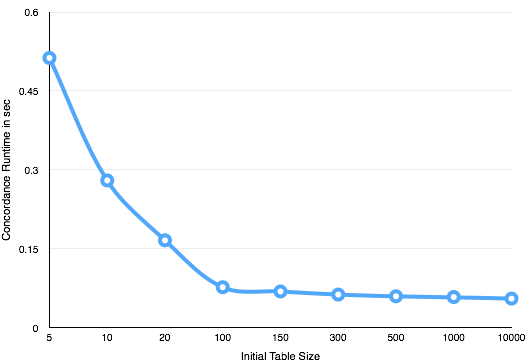
\includegraphics[width=0.75\textwidth]{sizing}
  \caption{Question 7 -- Hash Table Sizing Performance}
\end{figure}

%------------------------------------------------------

\end{document}

%%% Local Variables:
%%% mode: latex
%%% TeX-master: t
%%% End:
